
\section{Projeto do motor}

Da metodologia e dos requisitos expostos na seção~\ref{sec:motor_project}, foi gerada a geometria do motor para impressão 3D. A figura~\ref{fig:internal_profile} mostra a seção longitudinal projetada para o motor. Destaca-se o grande volume da câmara em comparação com a tubeira, devido à necessidade de haver estagnação de um fluxo intenso (ver seção~\ref{sec:result_validation}).

\begin{figure}[htbp]
    \centering
    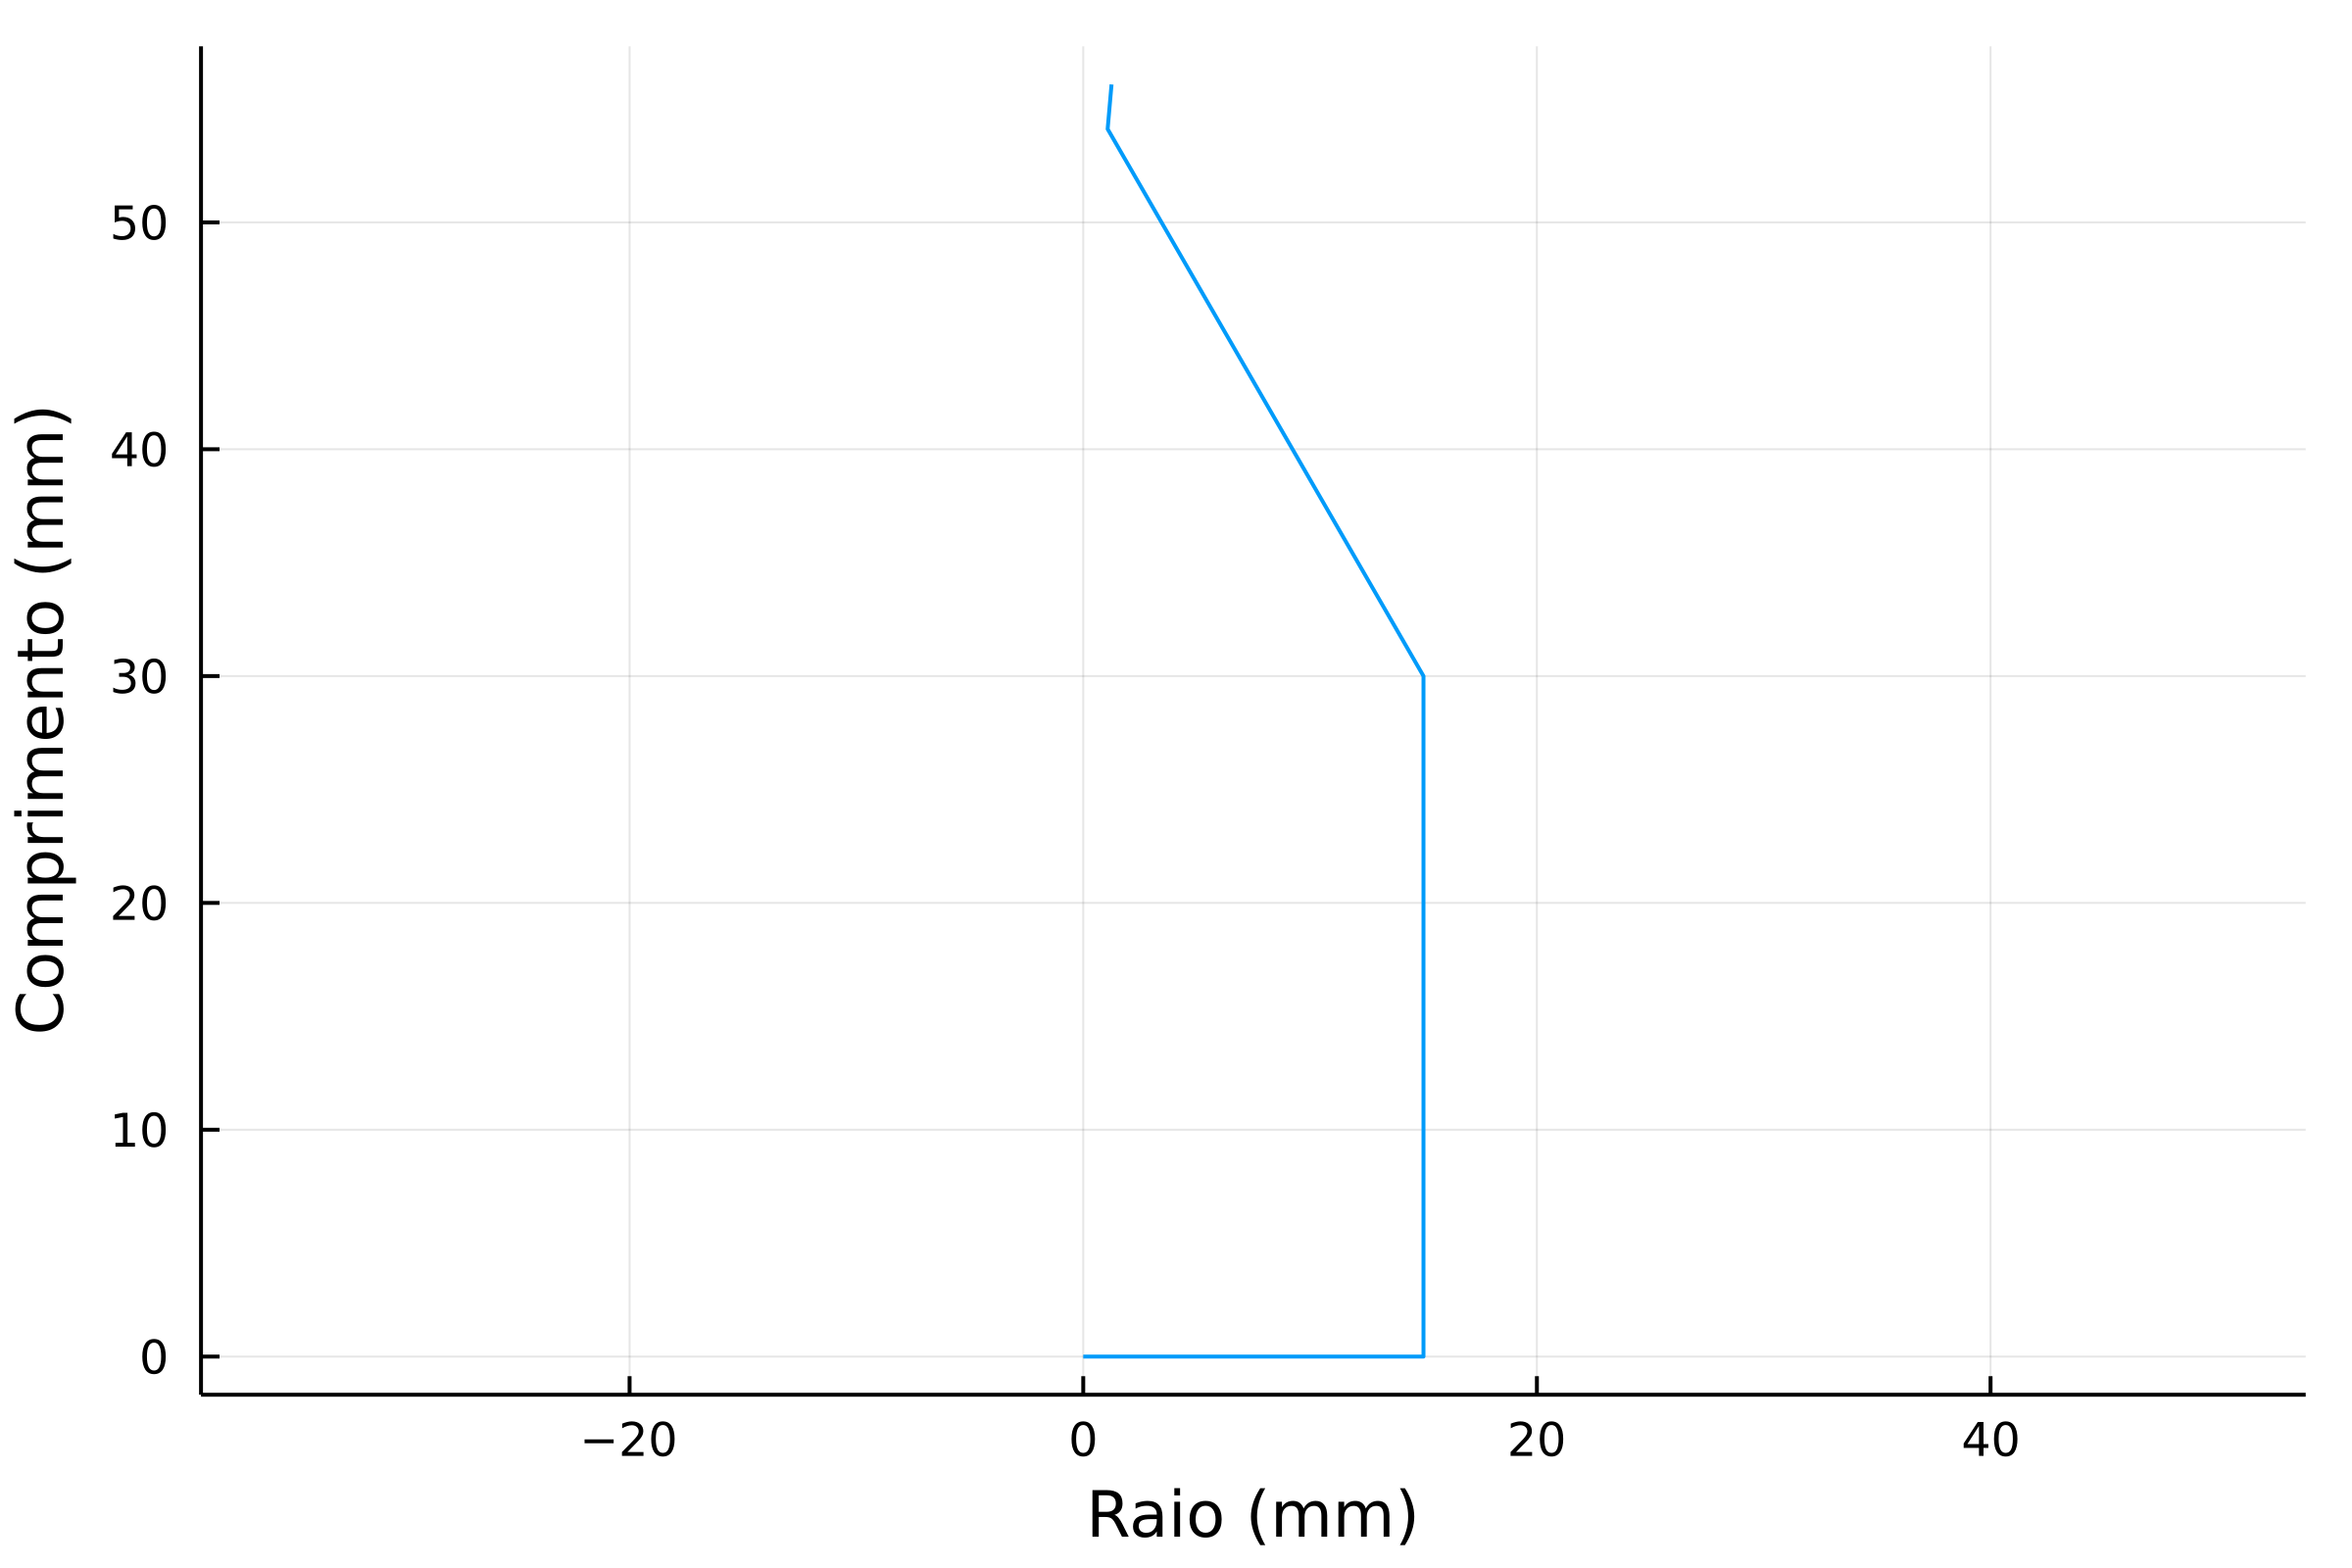
\includegraphics[width=\textwidth]{img/internal_profile.png}
    \caption{Perfil interno do motor projetado.}\label{fig:internal_profile}
\end{figure}

Os parâmetros propulsivos calculados para o motor foram:
\begin{itemize}
    \item \( \varepsilon = 1,35 \)
    \item \(C^* = 427,2\;\mathrm{m}\,\mathrm{s}^{-1}\)
    \item \(C_{F} = 1,10\)
\end{itemize}

Observa-se que o pequeno valor de razão de expansão é refletido na pequena tubeira exibida na figura~\ref{fig:internal_profile}. Foi obtido também um impulso específico de \(I_{sp} = 47,9s\)

\section{Validação do projeto do motor}\label{sec:result_validation}

\section{Projeto do sistema de \textit{jet vanes}}

\section{Caracterização do sistema em balança de três componentes}